\begin{figure*}[!p]
\centering
{\sffamily
\setlength{\tabcolsep}{4pt}
(a) \begin{tabular}{c|c|c|c|c|c|c}
\texttt{\#90} (400 nt) & Boltzmann & & struct. & energy gap & & \\
``Gladius'' & prob.\ $(\uparrow)$ & \NED$(\downarrow)$ & dist.\ $(\downarrow)$ & (kcal/mol) $(\downarrow)$ & \MFE & uMFE \\
\hline
EliteDesign ($N=500$) & {\boldmath$1.31 \times 10^{-11}$} & \textbf{0.081} & \textbf{20} & \textbf{7.9} & No & No \\
SamplingDesign & $4.77 \times 10^{-18}$ & 0.134 & 42 & 19.7 & No & No \\
\hline
Probability ceiling & $1.71 \times 10^{-8}$ & --- & --- & --- & --- & --- \\
\end{tabular}}\\[5pt]
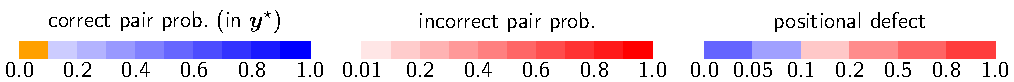
\includegraphics[width=\linewidth]{figures/structures/legend}\\[3pt]
{\sffamily
\begin{tabular}{@{}c@{\hspace{0.01\linewidth}}c@{\hspace{0.01\linewidth}}c@{}}
(b) Target \vecystar & (c) \MFE of EliteDesign ($N=500$) & (d) \MFE of SamplingDesign \\[2pt]
\raisebox{18pt}{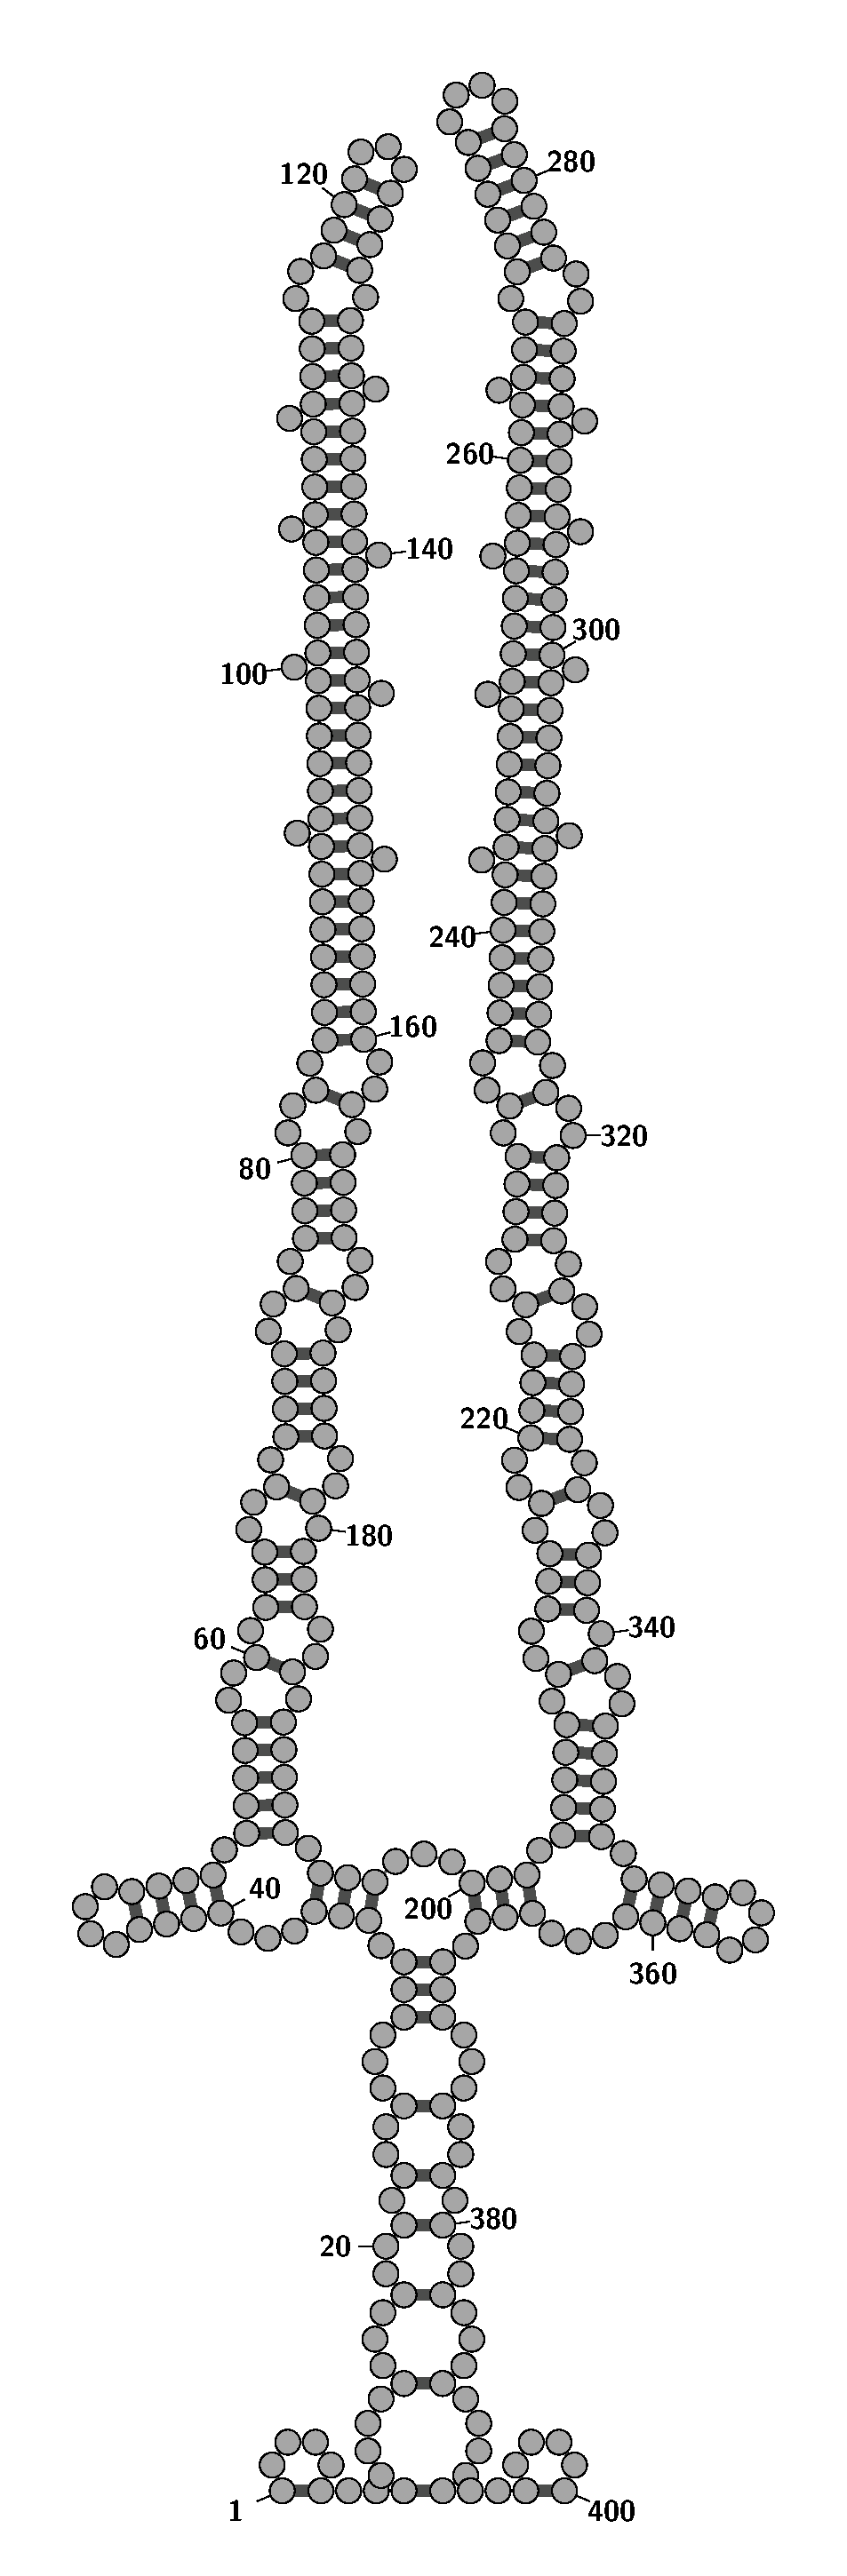
\includegraphics[scale=0.177,trim=36 10 36 36,clip]{figures/structures/target_90}} &
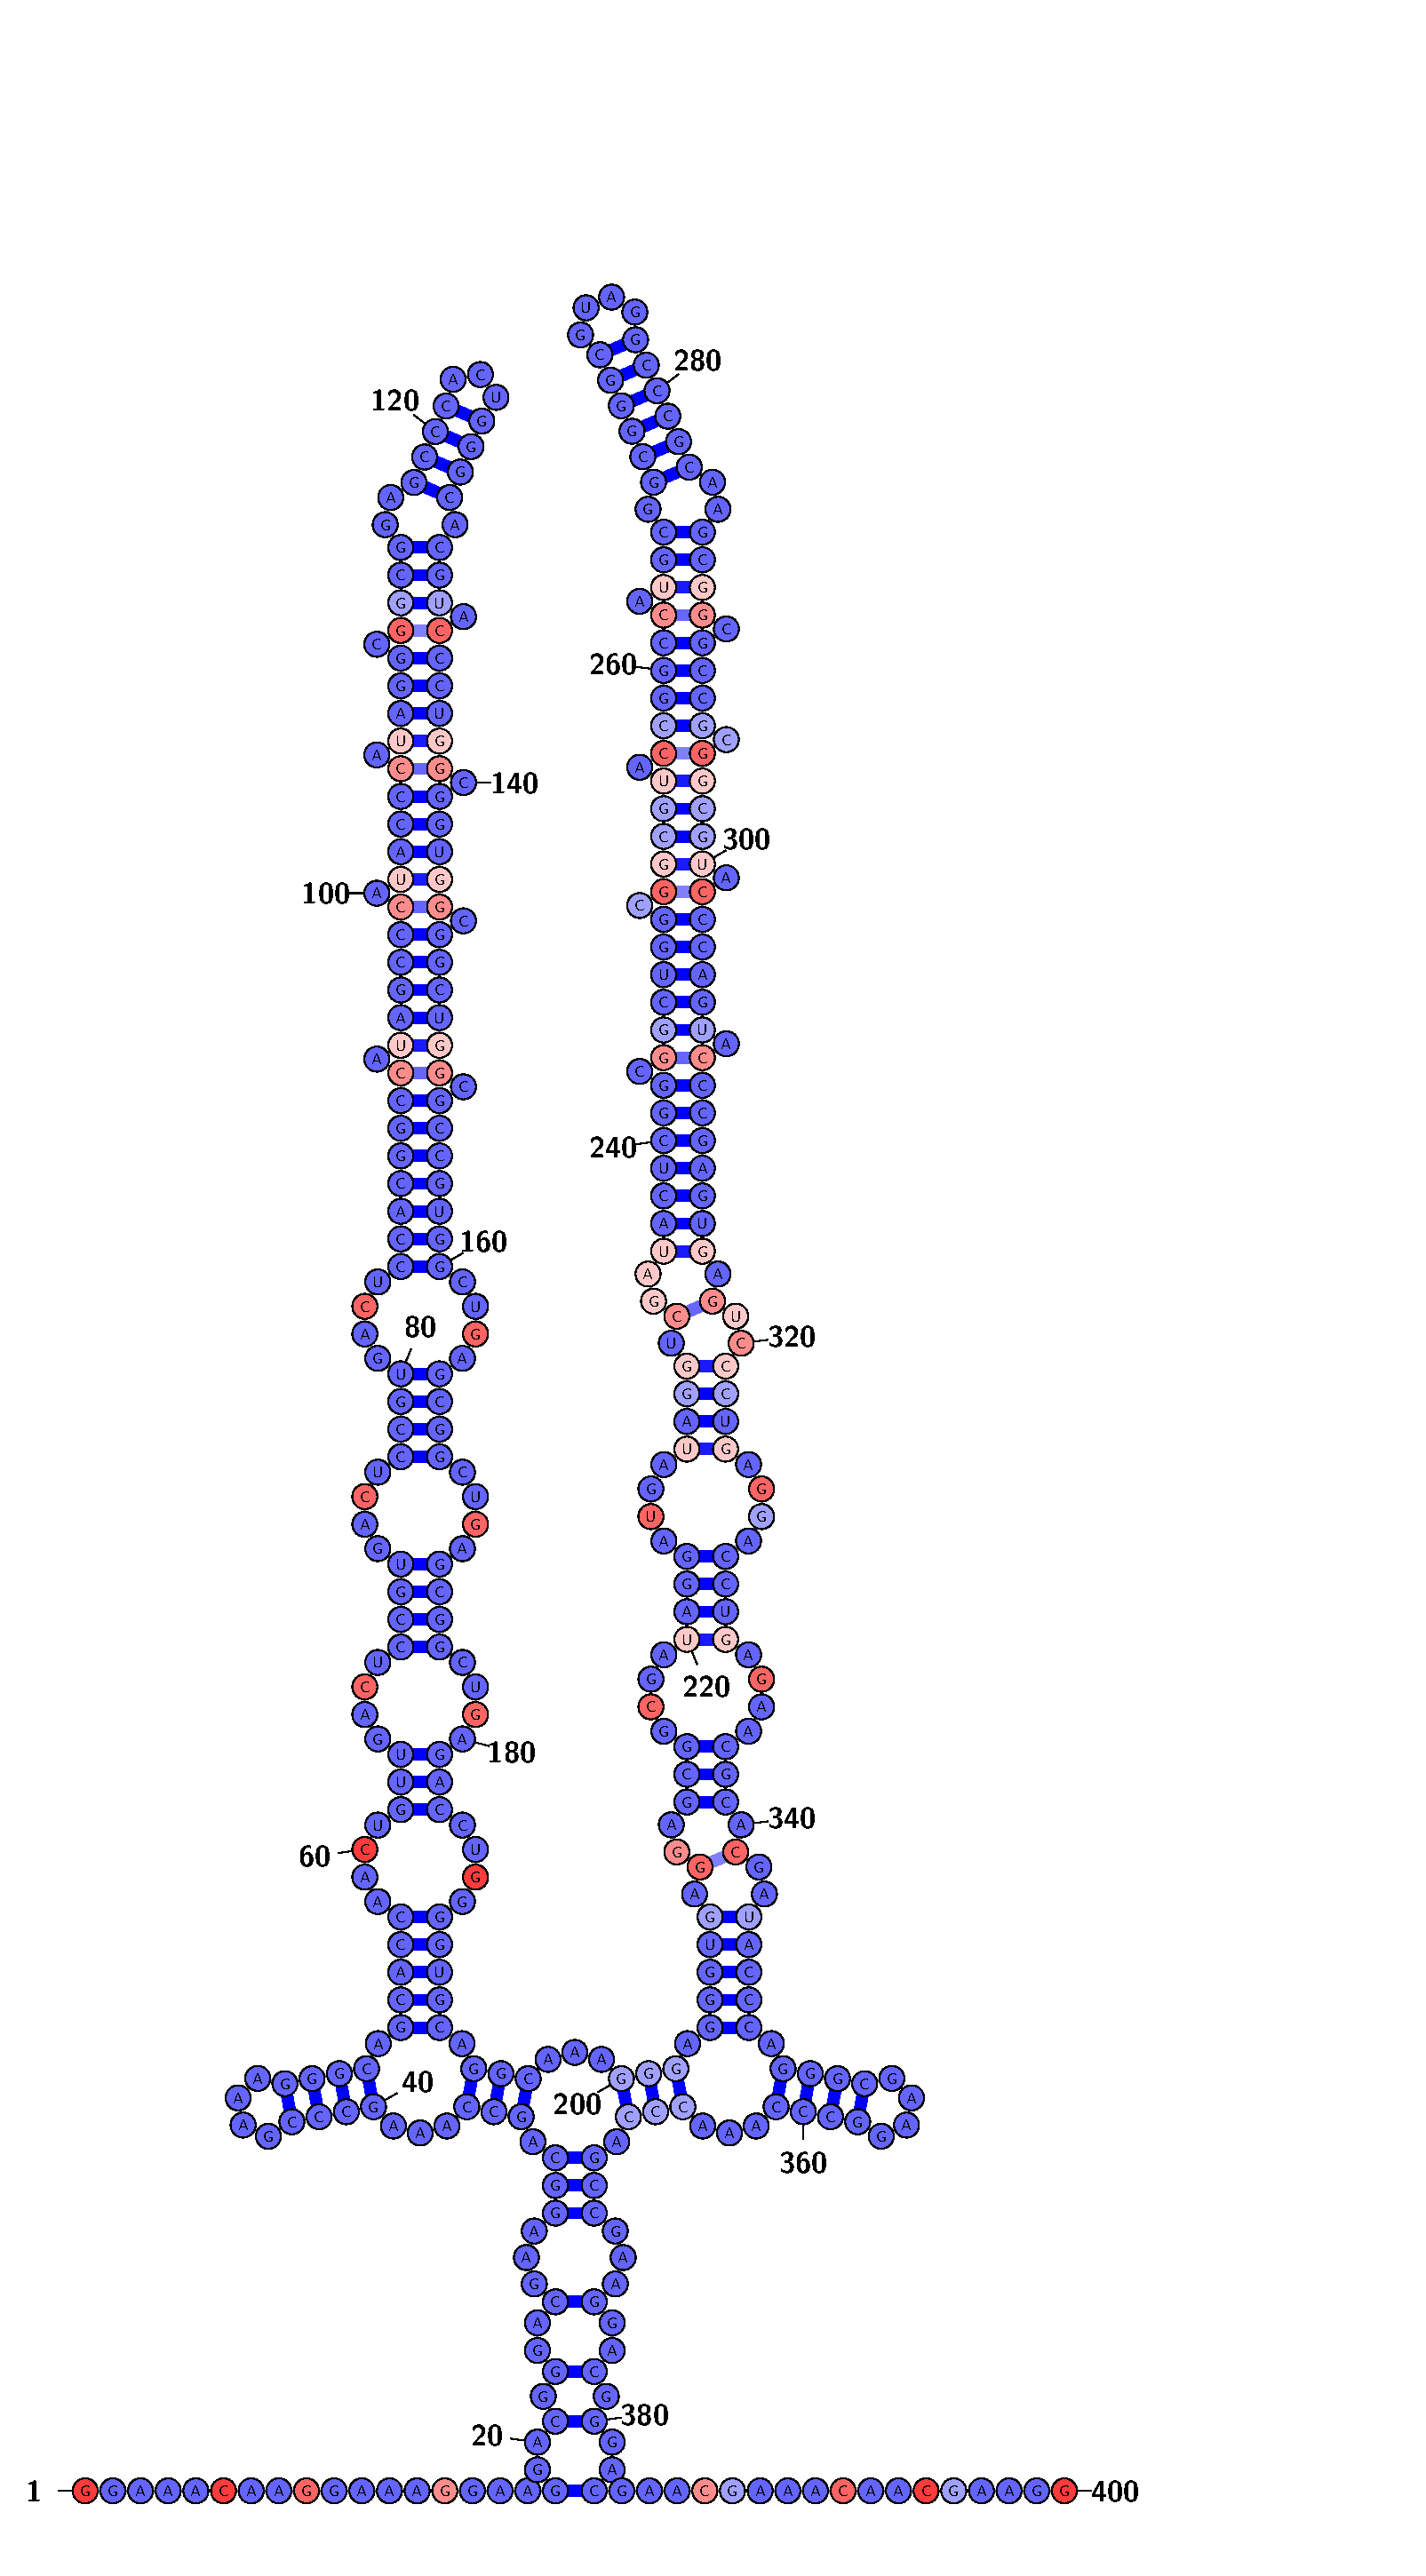
\includegraphics[scale=0.228,trim=12 36 152 151,clip]{figures/structures/structure_90_elite} &
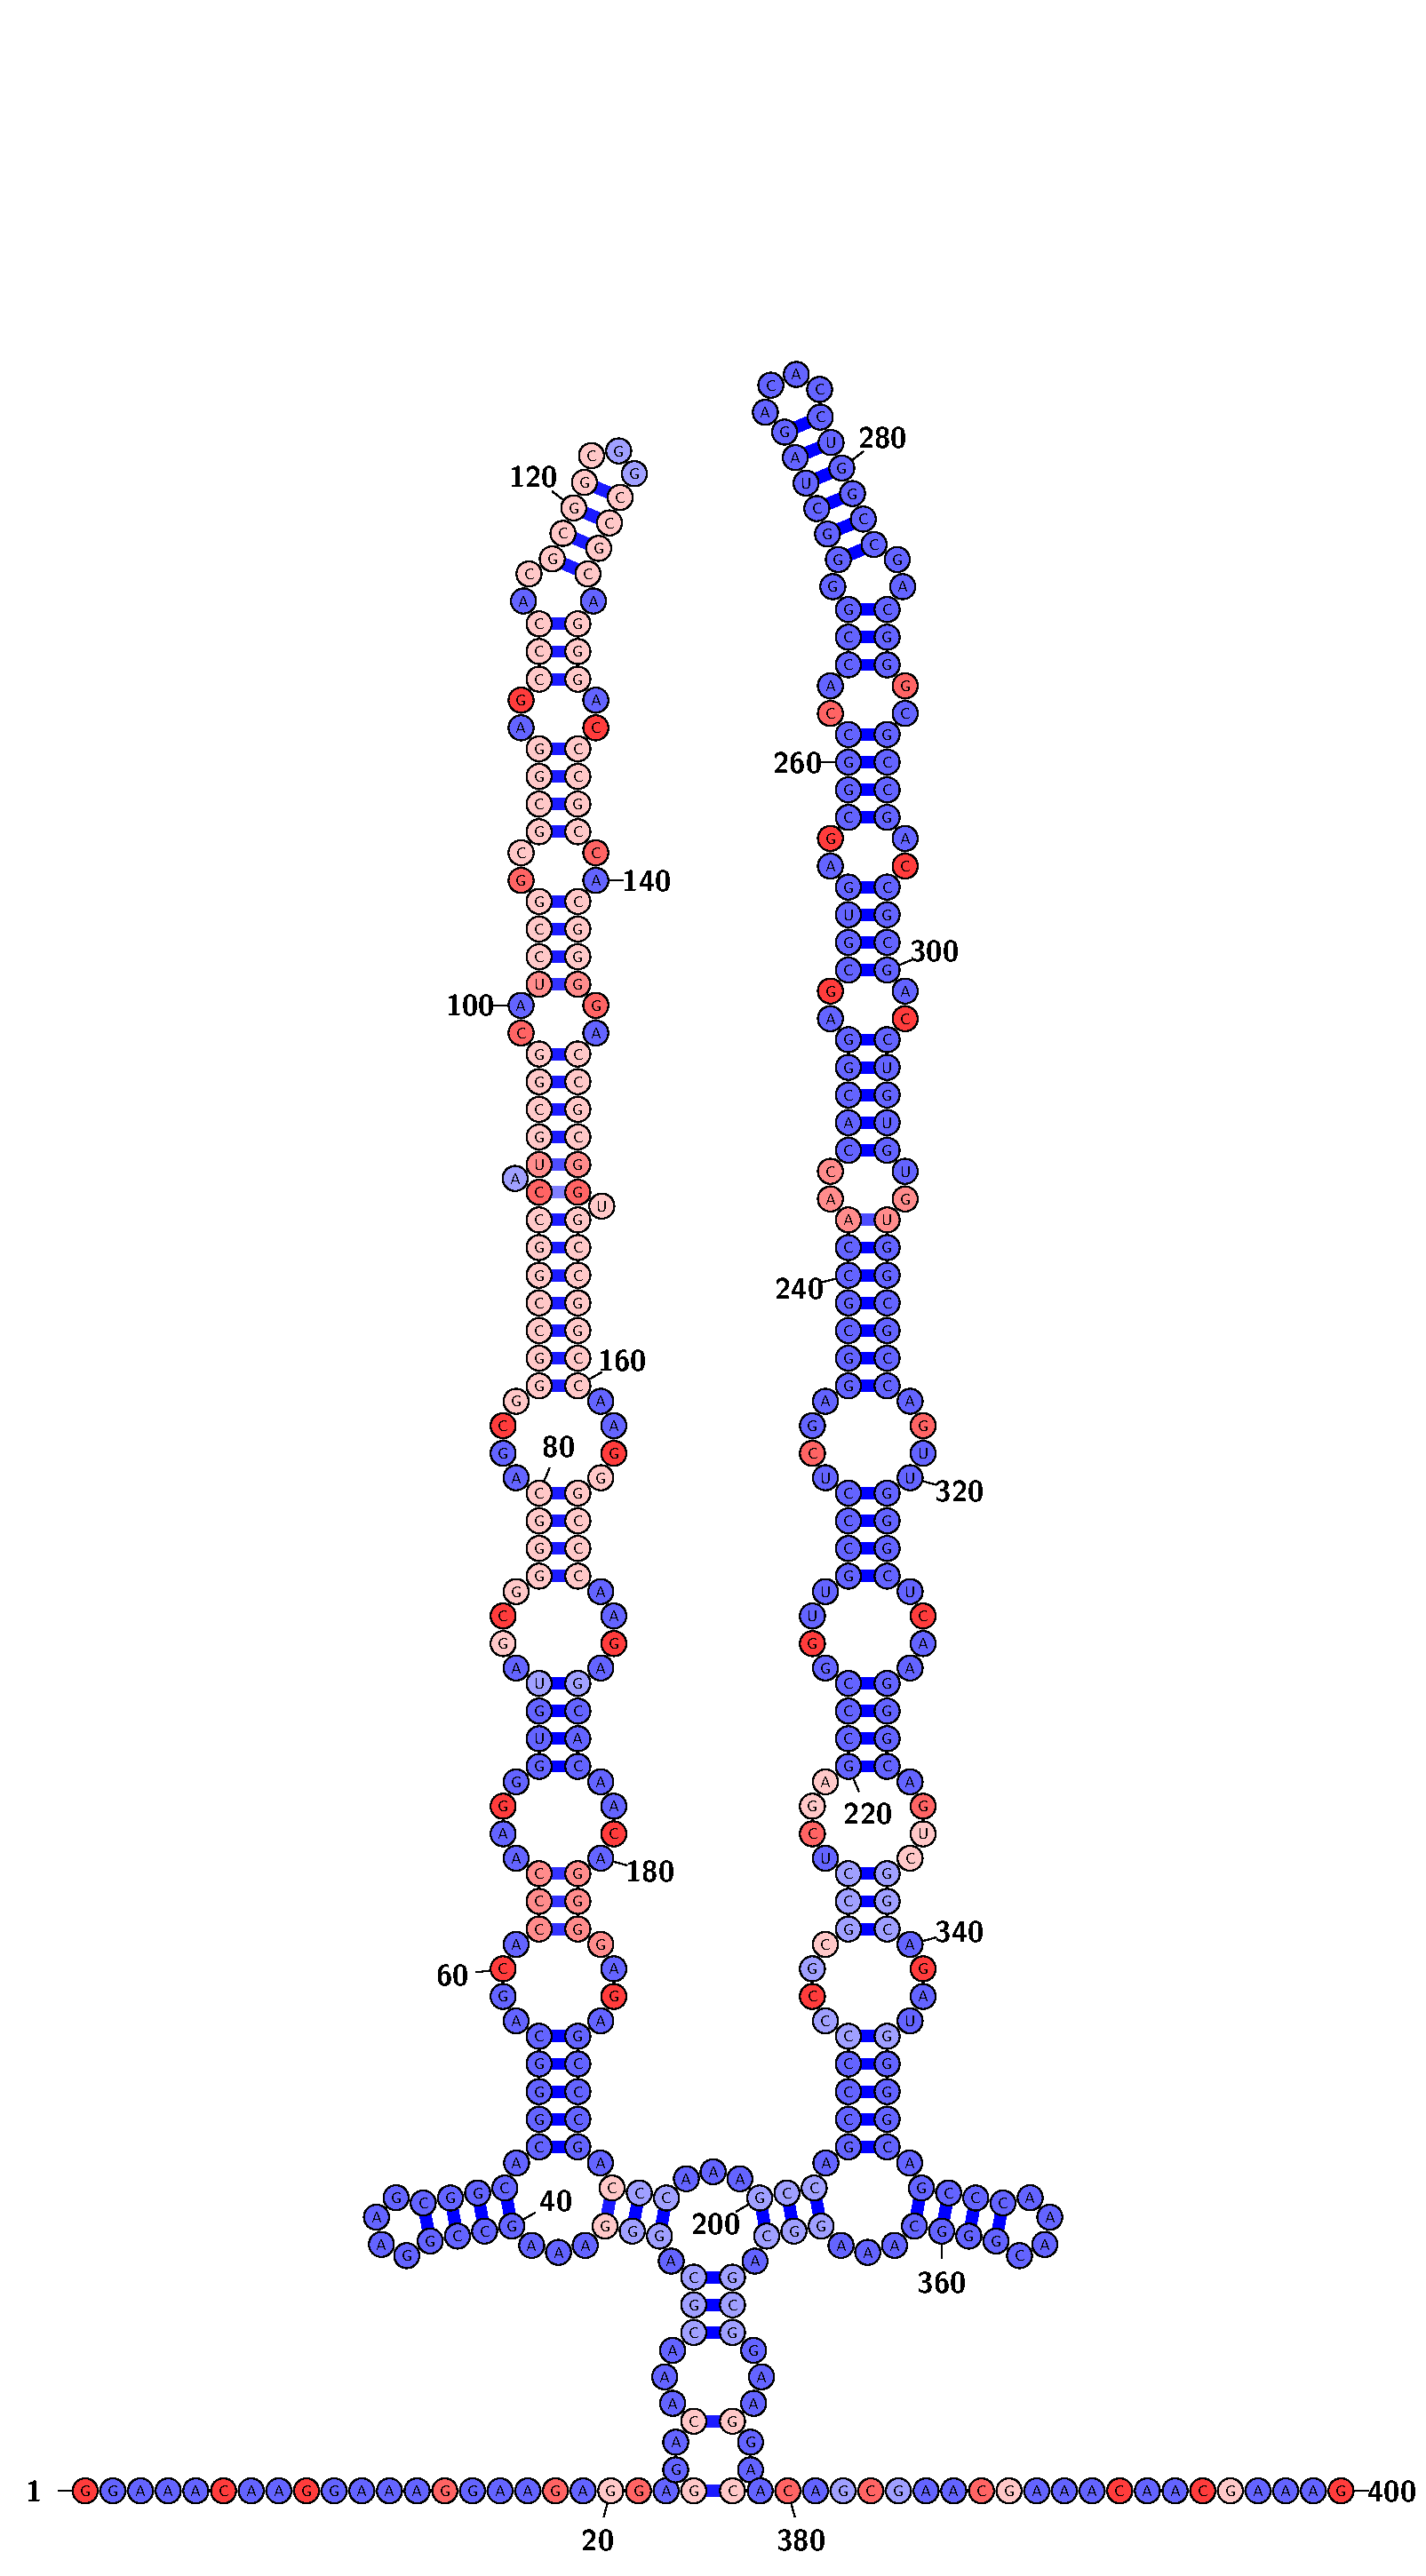
\includegraphics[scale=0.228,trim=12 11 3 192,clip]{figures/structures/structure_90_sampling}
\end{tabular}\\[3pt]
\begin{tabular}{@{}c@{\hspace{0.02\linewidth}}c@{}}
(e) Base-pairing probabilities, EliteDesign ($N=500$) & (f) Base-pairing probabilities, SamplingDesign \\[1pt]
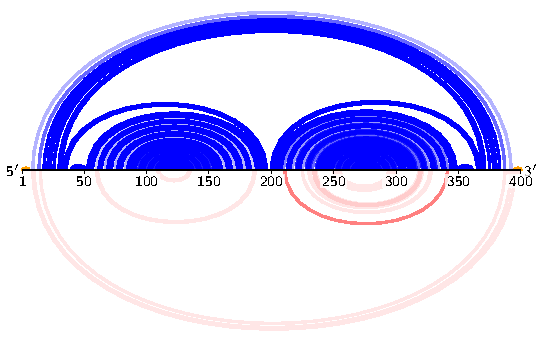
\includegraphics[width=0.44\linewidth,trim=0 8 0 4,clip]{figures/structures/arcs_90_elite} &
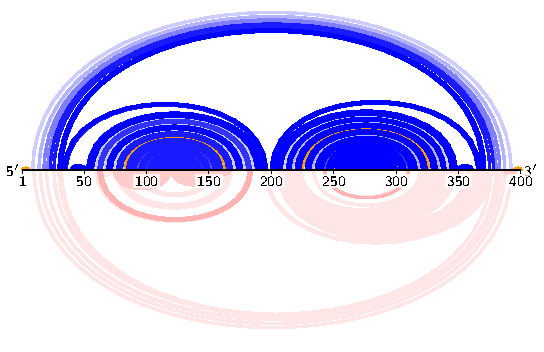
\includegraphics[width=0.44\linewidth,trim=0 8 0 4,clip]{figures/structures/arcs_90_sampling}
\end{tabular}}
\caption{This figure shows the sequences with the highest Boltzmann probability from EliteDesign ($N=500$) and SamplingDesign on Puzzle \texttt{\#90}, which is a proven undesignable puzzle. (a) The scores of each design and a probability upper bound on $p(\vecystar\mid\vecx)$~\citep{zhou2026}. (b) The target structure \vecystar. (c)--(d) The MFE structure of each design. Blue bonds belong to \vecystar and red bonds do not, darker bonds have higher probability, and nucleotides are colored by positional defect. (e)--(f) Base-pairing probabilities, where blue arcs are the pairs that match between a structure $\vecy'$ in the ensemble and \vecystar, orange arcs are matching pairs with a probability under 0.1, and red arcs are the pairs of $\vecy'$ that do not match \vecystar. Darker arcs have higher probability.}
\label{fig:eterna-structure-90}
\end{figure*}
